\documentclass[10pt,a4paper]{article}
\usepackage[utf8]{inputenc}
\usepackage[francais]{babel}
\usepackage[T1]{fontenc}
\usepackage{amsmath}
\usepackage{amsfonts}
\usepackage{amssymb}
\usepackage{graphicx}
\usepackage{epstopdf}
\usepackage{fancyhdr}
\pagestyle{fancy}
\usepackage{cite}
\usepackage{epsfig}


\renewcommand{\headrulewidth}{1pt}

\fancyhead[R]{} 
\fancyhead[L]{\textit{\leftmark}}

\addtolength{\hoffset}{-1.5cm}
\addtolength{\textwidth}{3.5cm}

\title{Projet MDI 343 \\
Systèmes de recommandation}
\author{Nicolas Keriven et Jean-Baptiste Alayrac}

\begin{document}
\maketitle

\hrulefill
\vspace{2cm}

\newcommand{\jel}{\textsc{Jellyfish} }
\renewcommand{\tablename}{TABLEAU}
% Si on veut mettre un abstract

%\renewcommand{\abstractname}{Résumé}
%\begin{abstract}
%
%
%\end{abstract}

% Figure 
%\begin{center}
%\begin{figure}[ht!]
%\includegraphics[width=\columnwidth]{fig/name.extension}
%\caption{\label{lab} titre}
%\end{figure}
%\end{center}

\newpage
\tableofcontents

\section*{Introduction}
\addcontentsline{toc}{section}{Introduction}
 
 Le challenge Netflix a mis en avant la problématique de créer de bons systèmes de recommandations. A l'heure où l'on est en mesure d'agréger énormément d'informations sur les utilisateurs, leurs préférences, leurs attitudes, il est légitime de se demander s'il est possible de traiter ces données afin d'améliorer l'expérience de l'utilisateur en lui proposant des produits qui vont lui plaire.
 
 Dans ce contexte beaucoup de méthodes ont été mises à l'épreuve afin de créer le système de recommandation le plus performant. Les techniques de factorisation de matrice se sont démarquées et ont notamment permis à l'équipe \textit{BellKor's Pragmatic Chaos} de remporter le prix d'un million de dollar décerné par Netflix \cite{koren}.
 
 On s'intéresse ici aux méthodes mathématiques et algorithmiques qui permettent de traiter efficacement un grand ensemble de notations afin de prédire les préférences d'utilisateurs pour des films.
 
 Dans un premier temps nous présenterons le problème et son cadre mathématique. Nous introduirons ensuite les algorithmes que nous avons implémenté afin de résoudre numériquement le problème. Enfin nous commenterons nos résultats en gardant en tête l'objectif de recommandation.
\newpage


\section{Présentation du problème et notations}

Le cadre général de la problématique de recommandation est de relier des utilisateurs à des produits. Dans cette partie nous présentons tout d'abord les méthodes les plus utilisées actuellement pour les système de recommandations avant de nous concentrer sur la méthode que nous avons approfondie.

\subsection{Différentes méthodes}

Actuellement, il existe deux principales approches afin de  créer un système de recommandation. La première approche est appelée \textit{content filtering} alors que la seconde est nommée \textit{collaborative filtering}

\subsubsection*{\textit{Content filtering} (ou filtrage par contenu)}

Cette méthode vise à caractériser la nature de chaque utilisateur ainsi que de chaque produit afin d'en dégager un profil le plus précis possible. Pour un utilisateur, cela peut être son pays d'origine, son âge... Pour un produit, par exemple un film, cela peut être son genre, son box-office... Les algorithmes ont alors pour tâche d'associer des profils d'utilisateurs avec des profils de produits. Le projet Music Genome Project, utilisé notamment dans la radio Pandora.com utilise de telles méthodes afin de proposer du contenu aux utilisateurs. Chaque musique est alors caractérisée par des centaines d'attributs assimilable à des "gènes". 


\subsubsection*{\textit{Collaborative filtering} (ou filtrage collaboratif)}

L'autre méthode se base essentiellement sur des avis passés (implicites ou explicites) d'utilisateurs à propos de produits. La méthode de \textit{collaborative filtering} analyse les liens qui existent entre utilisateurs et produits via la connaissance de votes passés afin de proposer de nouvelles associations utilisateur/produit. L'avantage principal de cette méthode par rapport à celle de \textit{content filtering} est qu'ici il n'y a nul besoin de connaître le produit ou les utilisateurs à priori. Par contre cette méthode connait le problème du \textit{cold start}, i.e., elle est incapable de traiter l'arrivée d'un nouveau produit ou d'un nouveau utilisateur. Afin de la faire fonctionner il faut posséder un nombre déjà conséquents d'avis de chaque utilisateurs et pour chaque produits.

Dans ce contexte de \textit{collaborative filtering} il existe à nouveau deux principales méthodes. La première est connue sous le nom de \textit{neighborhood method}, la deuxième se concentre autour de \textit{latent factor models}.

\begin{figure}[ht!]
\begin{center}
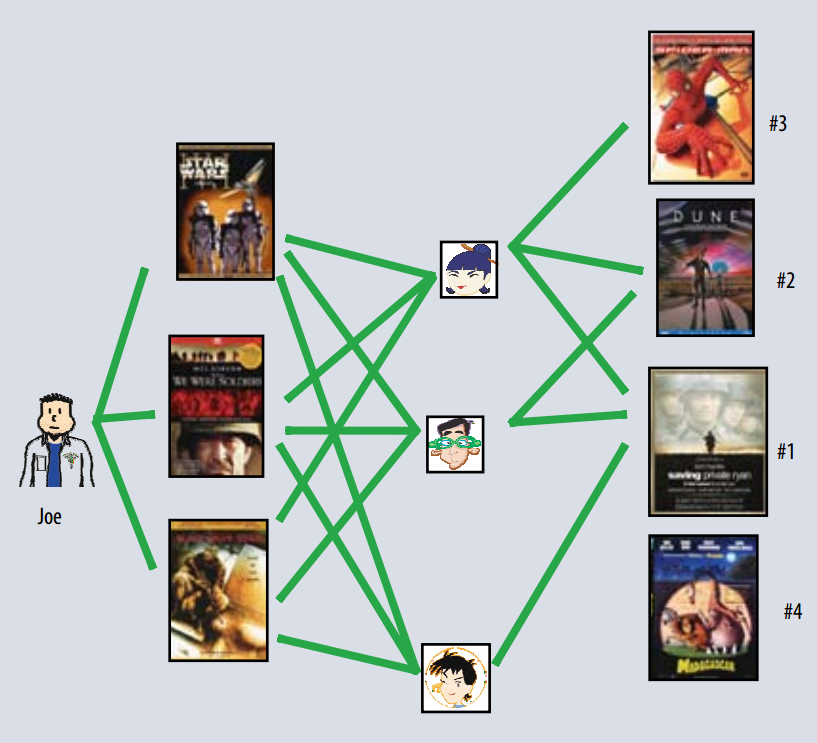
\includegraphics[height=5cm]{fig/neighboor_representation.png}
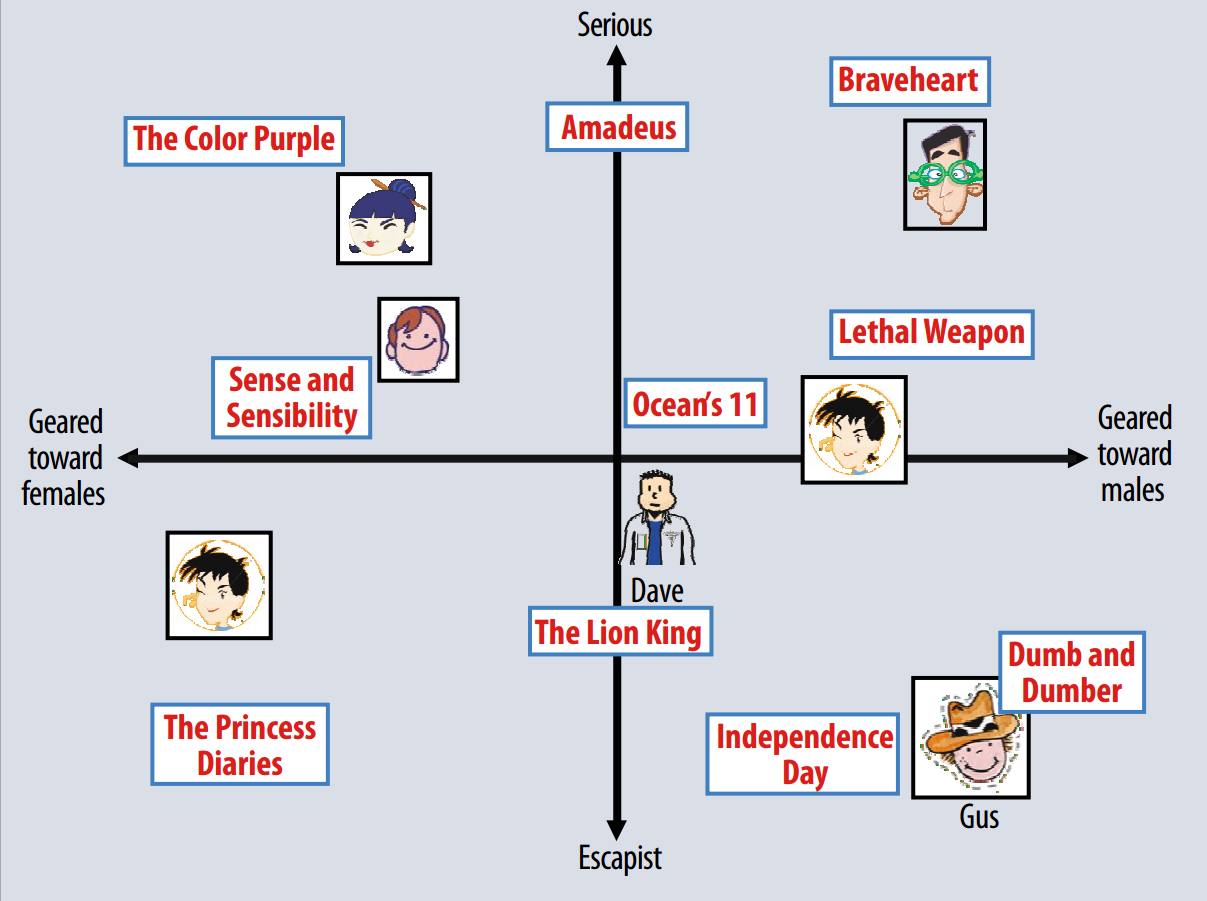
\includegraphics[height=5cm]{fig/factor_representation.png}
\caption{\label{nmet} A gauche : \textit{neighborhood methods}, A droite : \textit{Latent factor models}}
\end{center}
\end{figure}


\paragraph{\textit{Neighborhood methods}}

La principale idée est d'essayer de modéliser les relations qui existent entre les utilisateurs d'une part ou les produits d'autre part. Partons de l'approche produit. Supposons qu'on veuille prédire la note que va mettre un utilisateur à un nouveau produit A. On va alors regarder comment cet utilisateur a noté les produits identifiés comme étant des produits voisins de A, afin de prédire la note qu'il va mettre sur ce nouvel objet. Sur la gauche de la Figure \ref{nmet}, on a représenté l'approche utilisateur où l'on a d'abord trouvé un voisinage de l'utilisateur Joe afin de lui conseiller de nouveaux films (dans ce cas le premier film conseillé serait \textit{Il faut sauver le soldat Ryan}).

\paragraph{\textit{Latent factor model}}

Cette dernière approche est celle que nous avons choisi d'étudier plus en détails. L'idée derrière cette méthode est d'essayer est d'essayer de déterminer des \textit{facteurs latents} qui seront les dimensions d'un espace dans lequel on pourra plonger à la fois les utilisateurs et les produits. Cet espace sera directement déduit de la structure des votes qui est le lien entre utilisateurs et produits. L'idée ensuite est de pouvoir rassembler un utilisateur et un film qui seront proches dans cet espace. 

Ces facteurs latents peuvent être parfois interprétables. Par exemple une dimension pourront représenté le fait pour un film d'être une comédie. Les points maximaux seront alors considérés comme des comédies alors que les points minimaux pourront être des drames. La position d'un utilisateur sur cet axe témoignera alors de la propension de celui-ci à aimer ce genre. 

Cependant parfois ces facteurs ne sont pas interprétables directement, ce qui donne une certaine richesse au modèle. Cette méthode permet en effet de détecter des tendances qui n'aurait pas été prévisible à la main.

Sur la droite de la Figure 2 on a représenté cette approche pour 2 facteurs latents. De cela on peut prédire que l'utilisateur en haut à droite du graphique va certainement adorer le film \textit{Braveheart} alors qu'il va probablemnet détester le film \textit{The Princess Diaries}.

\subsection{Factorisation de matrice et notations}

Nous allons voir qu'une méthode afin de calculer ces facteur latents est de factoriser la partie connue de la matrice de notes $\textbf{M}$. On rappelle que $\textbf{M}_{u,i}$ est la note qu'a mis l'utilisateur $u$ au produit $i$ ($u$ pour \textit{user} et $i$ pour \textit{item}). Dans le cas où l'on a $n_u$ utilisateurs et $n_i$ produits cette matrice est donc de taille $n_u\times n_i$. Le gros obstacle est que cette matrice de notation est parcimonieuse, en effet bien souvent on ne possède qu'un certain nombre de produits pour lequel l'utilisateur a voté. Dans la suite on note $\Omega$ le set d'indices pour lequel la notation est connue. On a donc $|\Omega|\ll n_u\times n_i$. 

L'idée va alors être de trouver une matrice $\textbf{X}$ qui va être \textit{proche dans un certain sens} de l'information contenue dans la matrice $\textbf{M}$ et qui va pouvoir s'écrire de manière factorisé :

$$ \textbf{X} = LR $$

où $L \in \mathbb{R}^{n_u\times r}$ et $R \in \mathbb{R}^{r\times n_i}$ où $r$ est le nombre de facteurs latents que l'on recherche. Ainsi la ligne $u$ (resp. la colonne $i$) de la matrice $L$ (resp. $R$) va représenter la position dans l'espace des facteurs latents de l'utilisateur $u$ (resp. produit $i$). Le produit scalaire de ces deux vecteurs va donc représenter la propension de l'utilisateur $u$ a aimé le produit $i$. 

Maintenant essayons de décrire de manière plus mathématique la notion de \textit{proche dans un certain sens de l'information contenue dans $\textbf{M}$}. Il va donc falloir déterminer une fonction de coût $f$ d'attaches aux données sur la matrice $\textbf{X}$ en vue de se ramener à un problème classique d'optimisation. Une première idée serait de se dire que l'on pourrait écrire $f$ comme étant la moyenne empirique des écarts quadratiques entre $X_{ui}$ et la note $M_{ui}$. On aurait alors :

$$ f(\textbf{X}) = \frac{1}{| \Omega |}\sum_{(u,i)\in\Omega}\Vert X_{ui}-M_{ui} \Vert^2 $$

Cependant, avec cette représentation, on ne prend pas en compte le biais naturel qui existe dans nos données. En effet il est important de pouvoir modéliser le fait que certains utilisateurs sont plus sévères que d'autres pour noter les produits ou encore que certains produits sont parfois beaucoup mieux noté que la moyenne. Sans prendre en compte cela il devient difficile de modéliser les notes par un simple produit scalaire comme nous voulions le faire plus haut. Au lieu de représenter directement la note obtenue, on va préférer que le produit scalaire $X_{ui}$ représente l'écart à la note obtenue conte tenu du biais $b_{ui}$ que nous connaissons sur nos données :

$$b_{ui} = \mu + b_u  + b_i $$ 

où $\mu$ est la moyenne totale des notes, $b_u$ est la moyenne des notes décernés par l'utilisateur $u$, et $b_i$ est la moyenne des notes obtenues par le produit $i$. Tel quel $b_{ui}$ est déjà une sorte d'estimateur de la note que va mettre l'utilisateur $u$ au produit $i$. On verra dans la suite qu'il peut être intéressant de comparer nos résultats à ce système de recommandation très naïf. Ainsi on va réécrire notre fonction de coût d'attache aux données:

$$ f(\textbf{X}) = \frac{1}{| \Omega |}\sum_{(u,i)\in\Omega}\Vert X_{ui}+\mu + b_u  + b_i-M_{ui} \Vert^2 $$

Finalement notre problème de détermination de facteur latents peut s'écrire de la manière suivante :

\begin{equation}
\label{objectif}
 \text{minimiser } \frac{1}{| \Omega |}\sum_{(u,i)\in\Omega}\Vert X_{ui}+\mu + b_u  + b_i-M_{ui} \Vert^2 + P(\textbf{X})
\end{equation}


où $P$ est une fonction de régularisation qui permet de contrôler la complexité de la matrice $\textbf{X}$. Dans la suite nous allons décrire et comparer les algorithmes que nous avons utilisé afin de résoudre ce problème.

\section{Algorithmes}

\subsection{Descente de gradient stochastique}

% Parler de la différence entre tirage avec remise ou sans. Quel est l'avantage théorique d'une descente de gradient sto?

Lorsqu'on s'expose à des sets de données de très grande taille, le temps de calcul et la complexité de l'algorithme d'optimisation deviennent des contraintes que l'on ne peut pas négliger \cite{bottouSGD} \cite{bottou}. Dans ce contexte, l'algorithme de descente de gradient stochastique (noté SGD dans la suite) présente de nombreux avantages que ce soit du point de vue de la complexité mais aussi du point de vue de la performance.

Dans un souci de généralisation de notation nous remplaçons l'équation \eqref{objectif} par l'équation suivante, en supposant que la fonction de régularisation $P$ peut se décomposer en une somme sur les éléments de \textbf{X} (ce qui sera le cas en pratique) :

\begin{equation}
\label{objectif2}
 \text{minimiser } \frac{1}{| \Omega |}\sum_{(u,i)\in\Omega}l(X_{ui},M_{ui}) + P(X_{ui})
\end{equation}

\subsubsection*{Descente de gradient "usuelle"}

Les algorithmes de gradient classique calculent à chaque étape $t$ le gradient complet de la fonction objectif par rapport à $\textbf{X}_t$ et mette ensuite à jour $\textbf{X}_{t+1}$ en suivant différentes méthodes. L'une des plus efficaces en terme de convergence est la méthode de Newton qui sous certaines hypothèses parvient à une convergence quadratique. 

Cependant lorsque $| \Omega |$ devient très grand (ici 1 million voire 10 millions) il devient très coûteux de faire les étapes de calculs précédentes. On préférera alors une méthode plus simple comme l'algorithme SGD.

\subsubsection*{Descente de gradient stochastique}

Au lieu de calculer le gradient total à chaque itération de l'algorithme on va simplement calculer le gradient par rapport à un example (donc un couple $(u,i)$)  tiré aléatoirement. L'étape de mise à jour devient alors la suivante :

\begin{equation}
\label{grad}
X_{ui}^{t+1} = X_{ui}^t-\gamma_t\left(\nabla_Xl(X_{ui},M_{ui})+\nabla_XP(X_{ui})\right)
\end{equation}


En se ramenant au cas particulier de l'équation \eqref{objectif}, on voit que l'étape de mise à jour peut s'exprimer comme une mise à jour sur la $u$-ème ligne $L_u$ de la matrice $L$ et sur la $i$-ème colonne $R_i$ de la matrice $R$ (en supposant que $P$ peut se décomposer sur $L$ et $R$ ce qui sera le cas en pratique) :


\begin{eqnarray}
\label{grad1}
L_u & \leftarrow & L_u + \gamma_t\left(e_{ui}R_i^*-\nabla_L P_L(L_u)  \right) \\
R_i & \leftarrow & R_i  + \gamma_t\left(e_{ui}L_u^*-\nabla_R P_R(R_i)  \right)
\label{grad2}
\end{eqnarray}

où $e_{ui} = M_{ui} -  \mu - b_u  - b_i-L_{u}R_{i} $ est l'erreur de prédiction.

Le processus stochastique des exemples tirés au cours des itérations de l'algorithme est donc fortement corrélé à la manière dont on tire les exemples aléatoirement. Ici on espère que chacune des contributions (équation \eqref{grad}) se comportent comme la moyenne (descente de gradient usuelle), et ce malgré le bruit introduit par ces tirages.

\subsubsection*{Tirage avec remise}

Ici les tirages sont fait avec remise. De la sorte, en espérant que l'ensemble d'apprentissage est assez riche au sens de la distribution qu'il vise à représenter, on peut considérer qu'à chaque itération, les exemples sont tirés en suivant la véritable distribution des données. Intuitivement, on s'attend alors bien à ce que l'agrégation de toutes ces gradients ponctuels \eqref{grad} se comportent comme la moyenne (gradient total).

Des résultats de convergences ont été prouvés en supposant que le pas d'incrément $\gamma_t$ décroit suffisamment au cours des itérations. Le théorème de Robbins-Siegmund (1971) permet notamment de prouver la convergence presque sure de la méthode avec des hypothèses assez lâches.

Dans ce qui suit nous présentons une méthode qui permet de paralléliser cet algorithme afin de gagner du temps de calcul. On verra aussi que la méthode de tirage des exemples diffère de la méthode présentée ici. On s'efforcera alors de comparer ces deux méthodes.

\subsection{Algorithme parallélisé \jel }

Dans \cite{jelly}, les auteurs introduisent une version parallélisée de l'algorithme SGD, en remarquant qu'un grand nombre d'opérations sont indépendantes et peuvent être réalisées simultanément sans affecter le déroulement de l'algorithme et sans conflit. Cet algorithme, baptisé \jel, est essentiellement similaire à l'algorithme SGD et réalise successivement des opérations atomiques de descente de gradient selon une suite d'indices $(u_k,i_k)$. Outre l'implémentation, la seule différence entre les deux algorithmes repose dans la manière dont ces indices sont tirés.

\subsubsection*{Tirage sans remise}

Les équations de mise à jour \eqref{grad1} et \eqref{grad2} pour un couple d'indices $(u,i)$ affectent uniquement la $u$-ème ligne de $L$ et la $i$-ème colonne de $R$. Ainsi, deux de ces opérations pour des couples $(u,i)$ et $(u',i')$ tels que $u \neq u'$ et $i \neq i'$ sont totalement indépendantes: elles n'affectent pas les mêmes coefficients et peuvent être réalisées dans n'importe quel ordre, voire simultanément. C'est sur ce principe que repose l'algorithme \jel \cite{jelly}. Pour cela, le tirage des indices se fait \emph{sans remise}, contrairement à l'algorithme du gradient stochastique simple, et nous appellerons \emph{époque} le fait de parcourir une fois l'ensemble des données. Cet algorithme, similaire au gradient stochastique avec remise, a déjà été introduit sous le nom de descente de (sous-)gradient "incrémental" \cite{nedic}. Dans notre contexte, le tirage sans remise est plus une nécessité pratique qu'un véritable choix théorique: il est nécessaire de connaître à chacune de ces époques la séquence complète des indices à traiter afin de pouvoir paralléliser les opérations qui peuvent l'être.

Un véritable tirage sans remise se ferait via la sélection, avec une loi uniforme, d'une permutation sur $\Omega$. Cependant, une telle permutation peut rapidement devenir encombrante en mémoire et gloutonne en temps de calcul. Les auteurs de \jel  choisissent donc de tirer une permutation $\pi_u$ sur les utilisateurs et une permutation $\pi_i$ sur les items, et de sélectionner la permutation sur les couples $(\pi_u,\pi_i)$. Il est évident que l'on est loin de la loi uniforme: par exemple, en admettant que tous les utilisateurs et tous les items sont présents dans $\Omega$, il y a $(n_un_i)!$ permutations possibles sur $\Omega$, tandis qu'il existe seulement $n_u!n_i!$ de la forme $(\pi_u,\pi_i)$, ce qui est bien moindre. Si en pratique on s'attend à ce que cela ne fasse pas une grande différence, cela rend l'éventuelle analyse théorique d'un tel algorithme relativement subtile.

\subsubsection*{Description de l'algorithme}

Comme décrit dans la section précédente, à chaque époque l'algorithme tire uniformément une permutation $\pi_u$ sur les utilisateurs et une permutation $\pi_i$ sur les items. Suivant ces permutations, les données $(u,i) \in \Omega$ sont ensuite rangées dans des \emph{blocs} $C_{a,b}$, $1 \leq a,b \leq p$ de manière à ce qu'entre deux blocs $C_{a,b}$ et $C_{a',b'}$ tels que $a \neq a'$ et $b \neq b'$ toutes les opérations soient indépendantes, c'est-à-dire que pour tout $(u,i) \in C_{a,b}$ et $(u',i') \in C_{a',b'}$, on a $u \neq u'$ et $i \neq i'$. Pour cela, on pose simplement pour chaque couple $(u,i) \in \Omega$:

\begin{equation}\label{index}
a=\left \lfloor \frac{p}{n_u}(\pi_u(u)-1) \right \rfloor +1 \quad \quad b=\left \lfloor \frac{p}{n_i}(\pi_i(i)-1) \right \rfloor +1
\end{equation}

Au sein de chaque bloc, une étape de descente de gradient \eqref{grad} est réalisée sur chaque coordonnée. Le tirage sans remise est induit par les permutations: il est possible de traiter les données directement dans l'ordre dans lequel elles ont été "rangées" dans les blocs lorsque l'on parcoure $\Omega$ et que l'on applique \eqref{index}.

Il est possible de traiter en parallèle jusqu'à $p$ blocs ne s'intersectant pas en une \emph{étape}, puis de réaliser $p$ étapes afin de traiter toutes les données. Les blocs sont par exemple groupés selon les $p$ diagonales cycliques (Fig. \ref{blocs}). Ainsi, il est naturel de fixer $p$ au nombre maximum de processus pouvant être lancé (nombre de cœurs d'un processeur pour un ordinateur seul).

\begin{figure}
\centering
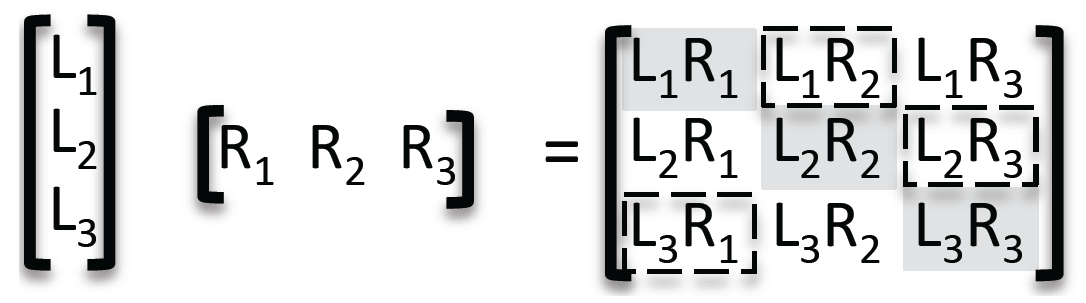
\includegraphics[width=0.8\textwidth]{fig/blocs}
\caption{Partition cyclique des blocs (pour question de simplicité, ici $\pi_u$ et $\pi_i$ sont les permutations identités). Les blocs surlignés de la même manière sont traités en parallèle. Schéma issu de \cite{jelly}.}
\label{blocs}
\end{figure}

\subsubsection*{Tirage sans remise, le retour}
Théoriquement, le tirage sans remise n'est pas à préférer au tirage avec remise. Ce dernier possède une vitesse théorique de convergence optimale \cite{jelly}\cite{bottou}, et lors d'un tirage sans remise une époque entière ne garantit nullement une plus grande proximité de la solution qu'après une seule étape de gradient \cite{nedic}. Cependant, plusieurs raisons portent à croire qu'un tirage sans remise est préférable pour des problèmes de taille importante. La plupart des analyses théoriques de l'algorithme de descente de gradient stochastique (avec remise) montrent que les bornes d'optimalité ne font pas intervenir la taille des données, ce qui est avantageux car adapté aux problèmes de grande taille, mais également limitant, le bruit résultant des choix aléatoires réalisés ne pouvant être contourné \cite{bottou}\cite{nedic}. Il est possible qu'en pratique un tirage sans remise évite certains de ces écueils. Intuitivement, une passe sur l'intégralité des données requiert en moyenne $n \log n$ tirages avec remise. Sur un problème de petite taille, le facteur $\log n$ est tout à fait négligeable, mais lorsque $n$ se compte en millions, cela peut résulter en un algorithme des dizaines de fois plus lent; le temps d'exécution s'accroît d'un ordre de grandeur non-négligeable.

Nous notons toutefois qu'il existe une version de l'algorithme extrêmement similaire \cite{gemulla_distri}, où le tirage se fait avec remise à l'intérieur de chaque bloc.

\subsubsection*{Détails d'implémentation}

De manière similaire au papier original, nous dévouons un processus entier à la permutation et l'ordonnancement des données. Il est lancé en parallèle des processus calculant le gradient à l'époque courante, et créé une copie des données permutées pour l'époque suivante (afin d'éviter les conflits de lecture). Ainsi, à tout instant deux copies des données sont gardées en mémoire.

Le papier original \cite{jelly} incite à dévouer plusieurs processus à cette permutation, quitte à accroître la mémoire utilisée. Cependant cela demande un niveau de contrôle de cette mémoire et de granularité quelque peu en dehors du cadre de ce projet -- la fusion des résultats des différents processus doit se faire intelligemment et rapidement, or de manière générale la mémoire partagée entre processus doit être pré-allouée et ne supporte pas les structures mutables comme les listes, etc. De plus, les auteurs dévouent deux processus sur douze à la permutation, et en pratique nous n'avons pas accès à d'aussi gros processeurs. Nous gardons donc dans la plupart des cas un seul processus alloué à cette permutation.

Cependant, dû à la non-mutabilité des données en mémoire partagée et au fait que la taille de chaque bloc dépend des permutations à chaque époque, l'ordonnancement des données se fait en deux étapes de temps de calcul à peu près égaux; pour calculer la taille de chaque blocs puis pour ranger les données. Ainsi, il est possible de diviser cet ordonnancement en deux processus: à l'époque $n$, un processus calcule les permutations et la taille des blocs pour l'époque $n+2$, un processus ordonne les données pour l'époque $n+1$, et les autres processus calculent les gradients. Selon le nombre de cœurs de la machine, il peut être possible de préférer affecter deux cœurs à l'ordonnancement des données, cependant lors de nos expériences sur nos machines relativement limitées, nous avons constaté que le calcul des gradients était systématiquement plus long, ainsi nous n'utilisons pas cette configuration.

\section{Résultats}

Nous présenterons nos résultats sous deux aspects. La première partie concernera la comparaison entre les deux algorithmes précédents en termes de précision par rapport à la fonction objectif et en termes de temps de calcul. On reviendra aussi sur la différence entre le tirage avec remise et sans remise.

 Dans la deuxième partie nous commenterons en détails les résultats obtenus sur la base de données du GroupLens Research \footnote{http://grouplens.org/datasets/movielens/}. Les résultats seront présentés sur la base de données qui comprend 1 million de notations de 6000 utilisateurs pour 4000 films. 

\subsection{Comparaison des deux algorithmes}
% Le nom peut changer :) 


\subsection{Résultats sur la base de données de films}
% Il faudra aussi parler des différents paramètres r...

Le premier point important est de constituer une base de test afin d'évaluer notre algorithme. Lors de la constitution de cette base de tests, il faut prendre soin de ne pas retirer toutes les notes d'un même utilisateur ou toutes les notes d'un même film. Dans le cas contraire on perd toute l'information sur cet utilisateur ou sur ce film. La stratégie que nous avons adopté est de retirer $n$ notes par utilisateurs en espérant que toutes les notes d'un même film ne soient pas retirées (une vérification avant chaque test est nécessaire). En pratique $n=1,2$, ce qui nous permet d'avoir une base de test assez conséquente.

\subsubsection*{Critère d'évaluation}

\paragraph{RMSE}

Afin d'évaluer la pertinence de notre algorithme nous avons regardé plusieurs facteurs. Le premier critère chiffrée est le RMSE (pour \textit{Root Mean Square Error}):

$$ \text{RMSE} = \sqrt{\frac{1}{|\Omega_{\text{test}|}}\sum_{(u,i)\in \Omega_{\text{test}}} |X_{ui}+b_{ui}-M_{ui}|^2} $$

Par rapport à la simple erreur moyenne, ce critère permet de pénaliser plus les erreurs qui sont vraiment loin de la  valeur attendue. On accepte avec une bonne tolérance qu'un algorithme se trompe d'un point sur une note de 5, par contre on sera totalement insatisfait si l'algorithme se trompe de 3 points. Le rapport de mécontentement n'étant pas linéaire, ce critère est plus pertinent que la simple erreur moyenne.


Nous avons aussi choisi ce critère parce qu'il est le critère d'évaluation du challenge Netflix. Pour information sur la base de test Netflix le RMSE avec le prédicteur naïf par la moyenne est de 1.02. Avant la compétition Netflix parvenait à un RMSE de 0.95. Après plusieurs années de compétition le RMSE est passée à 0.85. Il est important de garder cela en tête lorsque nous comparerons les résultats de notre algorithme avec ceux du prédicteur naïf. Ce critère sera donc utile pour comparer différents paramètres, ou la performance des deux algorithmes étudiés ici. 

 Sur notre base de test, le RMSE "naïf" est de 0.9598.

\paragraph{Histogramme d'erreur} Afin de visualiser mieux ce que peut représenter le chiffre précédent, nous avons affiché l'histogramme des erreurs en comparant un résultat de notre algorithme avec le prédicteur naïf par la moyenne. Un exemple d'un tel histogramme est donnée en Figure \ref{histo_best}.

\paragraph{Affichage des facteurs latents}

Enfin un dernier critère d'évaluation a été d'essayer de visualiser la pertinence attendue des facteur latents. Pour cela nous avons reproduits des figures similaires à la Figure \ref{nmet}, en représentant des films en deux dimensions répartis aux extrêmes dans l'espace des facteurs latents. Cependant il faut d'ores et déjà savoir que tout les facteurs latents ne seront pas facilement interprétables en termes de genre cinématographique, de box office...

\subsubsection*{Résultats}

Dans le Tableau \ref{RMSE_vs_r} on donne le RMSE obtenu pour différentes valeurs de $r$. On rappelle que $r$ est le rang de la matrice $X$, ou encore la dimension de l'espace des facteurs latents. On rappelle aussi que ce résultat est à comparer au RMSE naïf qui vaut $0.9598$.

\begin{table}[h]
\begin{center}
   \begin{tabular}{|c|c|c|c|c|c|c|}
  	\hline
  	\textbf{Dimension $r$} & \multicolumn{2}{c|}{10} & \multicolumn{2}{c|}{50} & \multicolumn{2}{c|}{100} \\
  	\hline
  	\textbf{Algorithme} & SGD & \jel & SGD & \jel & SGD & \jel \\
  	\hline
  	\textbf{RMSE}  & 0.9146  &  & 0.9114 & & 0.9042 &\\
  	\hline
\end{tabular}
\end{center}
\caption{\label{RMSE_vs_r} Valeurs du RMSE pour différentes valeurs de $r$}
\end{table}

En Figure \ref{histo_best}, on donne l'histogramme des erreurs obtenu pour le plus bas RMSE. En bleu, on visualise les prévisions de notre algorithme d'optimisation et en vert on peut voir les prédictions de la moyenne simple ($\textbf{X}=0$). 

% A remplacer par le meilleur!


%\begin{figure}
% \begin{minipage}[b]{.46\linewidth}
%  \centering\epsfig{figure=fig/hist.eps,height=5cm}
%  \caption{Histogramme d'erreur \label{histo_best}}
% \end{minipage} \hfill
% \begin{minipage}[b]{.46\linewidth}
%  \centering\epsfig{figure=fig/graph_best.eps,height=5cm}
%  \caption{Part de bonnes prédictions \label{graph_best}}
% \end{minipage}
%\end{figure}

\begin{figure}[ht!]
\begin{center}
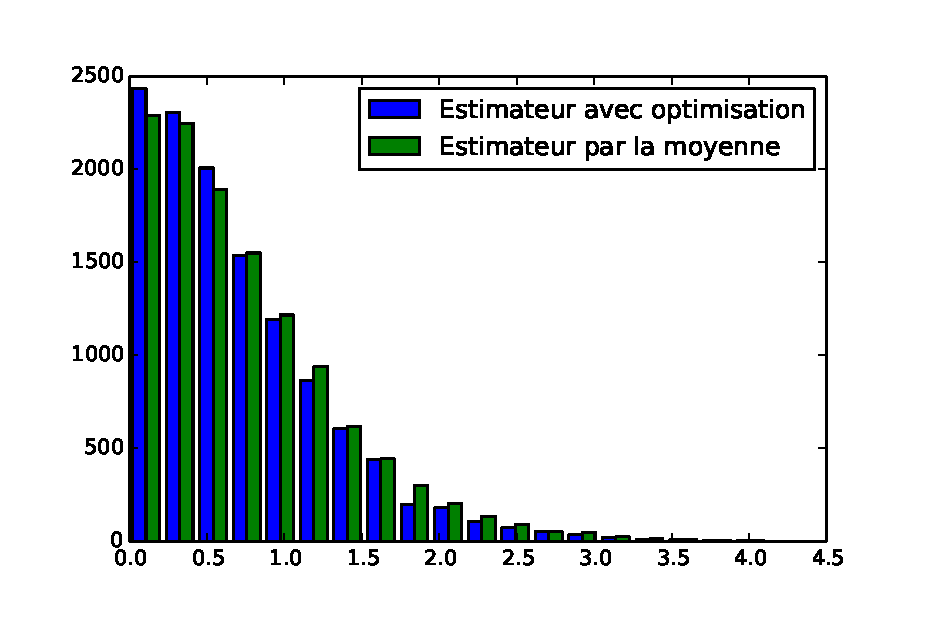
\includegraphics[height=5cm]{fig/hist.eps}
\caption{\label{histo_best} Histogramme d'erreur}
\end{center}
\end{figure}


En Figure \ref{graph_best} on donne pour chaque note (comprise entre 1 et 5) la proportion de notes où notre algorithme ne s'est pas trompé pour le meilleur RMSE. En comparaison on donne aussi la prédiction de l'algorithme naïf. Ce graphique permet une visualisation un peu plus parlante des résultats de notre algorithme en vue de créer un système de recommandation. 

\begin{figure}[ht!]
\begin{center}
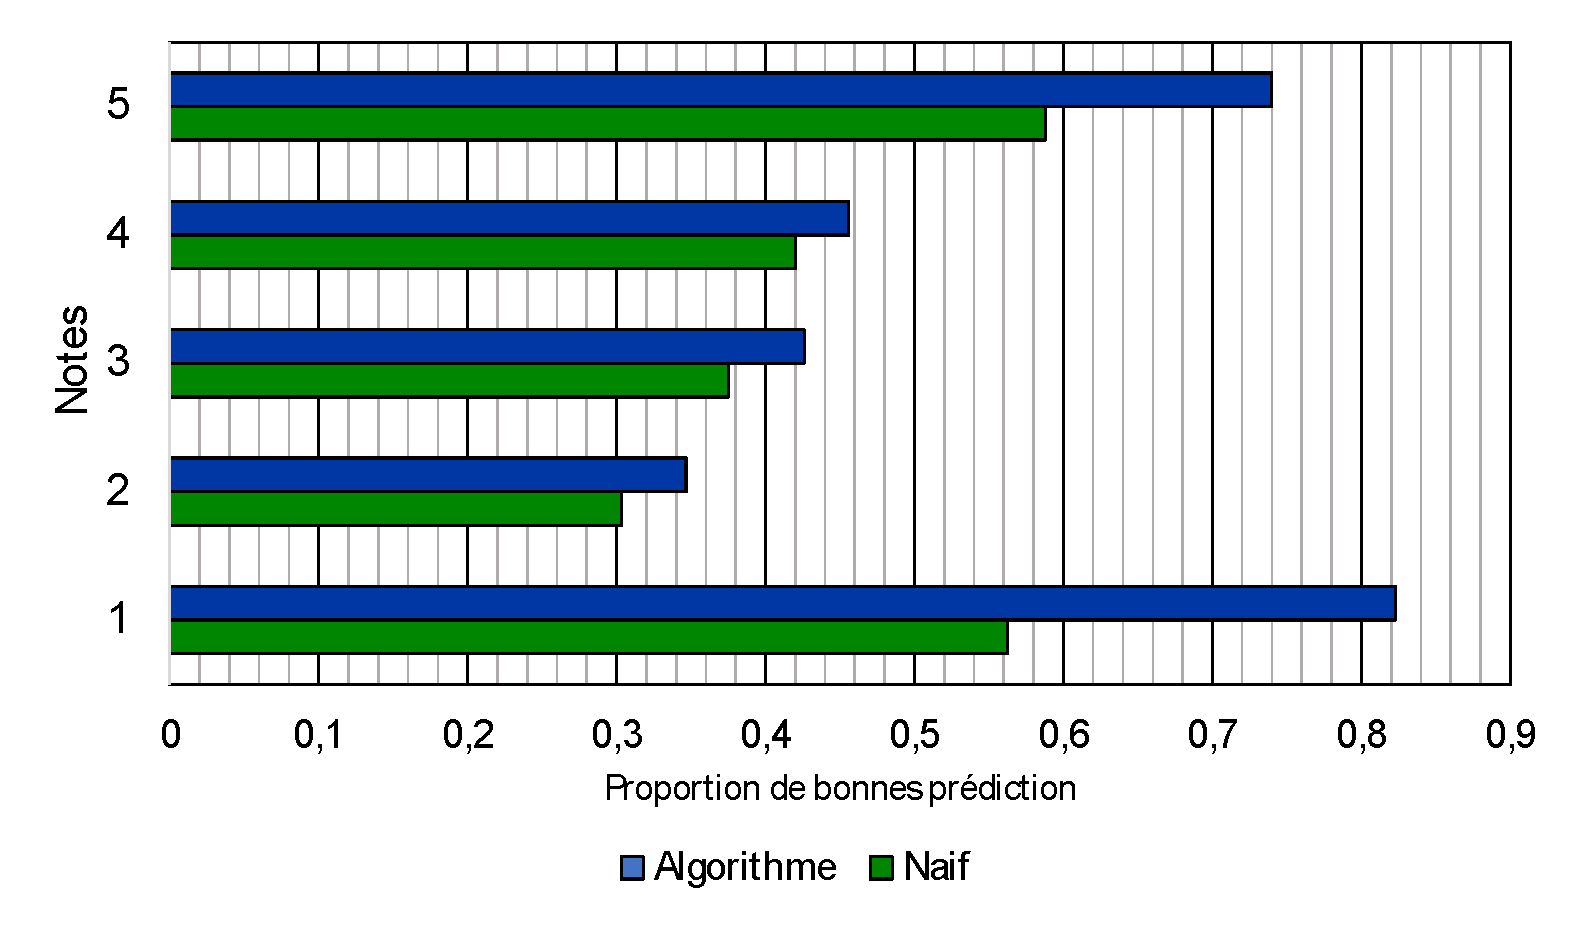
\includegraphics[height=5cm]{fig/graph_best.eps}
\caption{\label{graph_best} Proportion de bonnes prédiction en fonction de chaque note}
\end{center}
\end{figure}


\subsubsection*{Espace des facteur latents}

Nous voyons dans le tableau \ref{RMSE_vs_r}, que la performance de notre algorithme augmente avec $r$, du moins au début (nous n'avons pas testé avec des $r$ trop grand mais le risque ensuite devient l'overfitting). Il est alors intéressant de se pencher sur les espaces engendrés par notre algorithme. 

% Blabla avec figure!

\subsubsection*{Commentaires}

Dans cette partie nous apportons un regard critique sur les résultats présentés précédemment en essayant de replacer cela dans le contexte de la recommandation. 

% Partie positive
Comme nous pouvons le voir dans le tableau \ref{RMSE_vs_r}, notre algorithme parvient à battre la méthode naïve qui reviendrait à prédire n'importe quelle note par la moyenne des notes passées. De plus dans le but de réaliser un algorithme de recommandation on a envie que notre algorithme prédise de manière efficace surtout les notes extrêmes afin, d'une part de proposer des produits à l'utilisateur dont on est sûr qu'ils vont plaire, et d'autre part d'être en mesure de bien prévoir ce que l'utilisateur va détester. En ce sens le graphique de la Figure \ref{graph_best} est intéressant parce qu'on voit que notre algorithme est bien plus efficace que la méthode naïve pour ce qui est de prédire les notes extrêmes. Pour la note 5, nous avons 74 $\%$ de bonnes prédictions avec notre méthode contre 59 $\%$ pour la méthode naïve. Pour la note 1 nous avons 82 $\%$ de bonnes prédictions avec notre approche contre 56 $\%$ pour la prédiction par la moyenne. En ce sens nous pouvons dire que l'approche étudiée ici fonctionne assez bien pour faire de la recommandation. Il semblerait donc que l'on réussisse à capter de l'information sur les goûts et les préférence des utilisateurs.

%Partie négative
Cependant on est aussi en droit de se demander si, du point de vue de l'utilisateur, l'amélioration de prédiction est réellement intéressante. En reprenant l'exemple du projet Netflix, on peut noter que la bonne prédiction de notes au dessus de 3 étoiles est de 98.9 $\%$ pour l'algorithme qui a décroché le prix de 1 million de dollar contre 94.4 $\%$ pour l'algorithme naïf. On peut alors se demander si l'amélioration de l'expérience de l'utilisateur est vraiment intéressante. Beaucoup de progrès reste encore à faire afin de comprendre et de modéliser les goûts humains. Cette idée permet de relativiser quant aux résultats modestes de nos algorithmes.

\section*{Conclusion}

\newpage

\bibliographystyle{unsrt}
\bibliography{biblio}
\end{document}